\section{Hardware}

\subsection{Zielsetzung des Hardwareaspekts}
Entscheident beim Aufbau eines Supercomputers ist
es die Faktoren Platzbedarf, Rechengeschwindigkeit und Kühlung 
in eine gleichgewicht zu bringen. Bei einem grünen Supercomputer 
muss darüberhinaus auch die Energeeffizienz beachtet werden,
welche maßgeblich durch den Aufbau des Clusters beeinflusst wird.

%Der zweite wichtige Aspekt beim Aufbau eines unkonventionellen 
%Supercomputers ist der physikalische Aufbau des Computers.
%Hierbei muss man darauf achten ein Gleichgewicht zwischen den Faktoren 
%Energieverbrauch, Rechengeschwindigkeit, und Kühlung zu finden.
%Zusätzlich soll unabhängig von der Größe des Clusters eine
%einfache Lösung für das Monitoring bereitgestellt werden.

\subsection{Vorbereitung und Hardwareauswahl}
Die für die Kühlung des Clusters benötigte Energie, und
somit auch die Energeefizienz, ist eng mit der Anordnung der Rechenknoten
verbunden. Daher wurden zu Beginn einige Modelle konstruiert 
um diese zu Optimieren und einen zielgerichteten ablauf der Konstruktion
zu gewährleisten.~\\
\begin{minipage}{0.45\textwidth}
\begin{figure}[H]
  \centering
    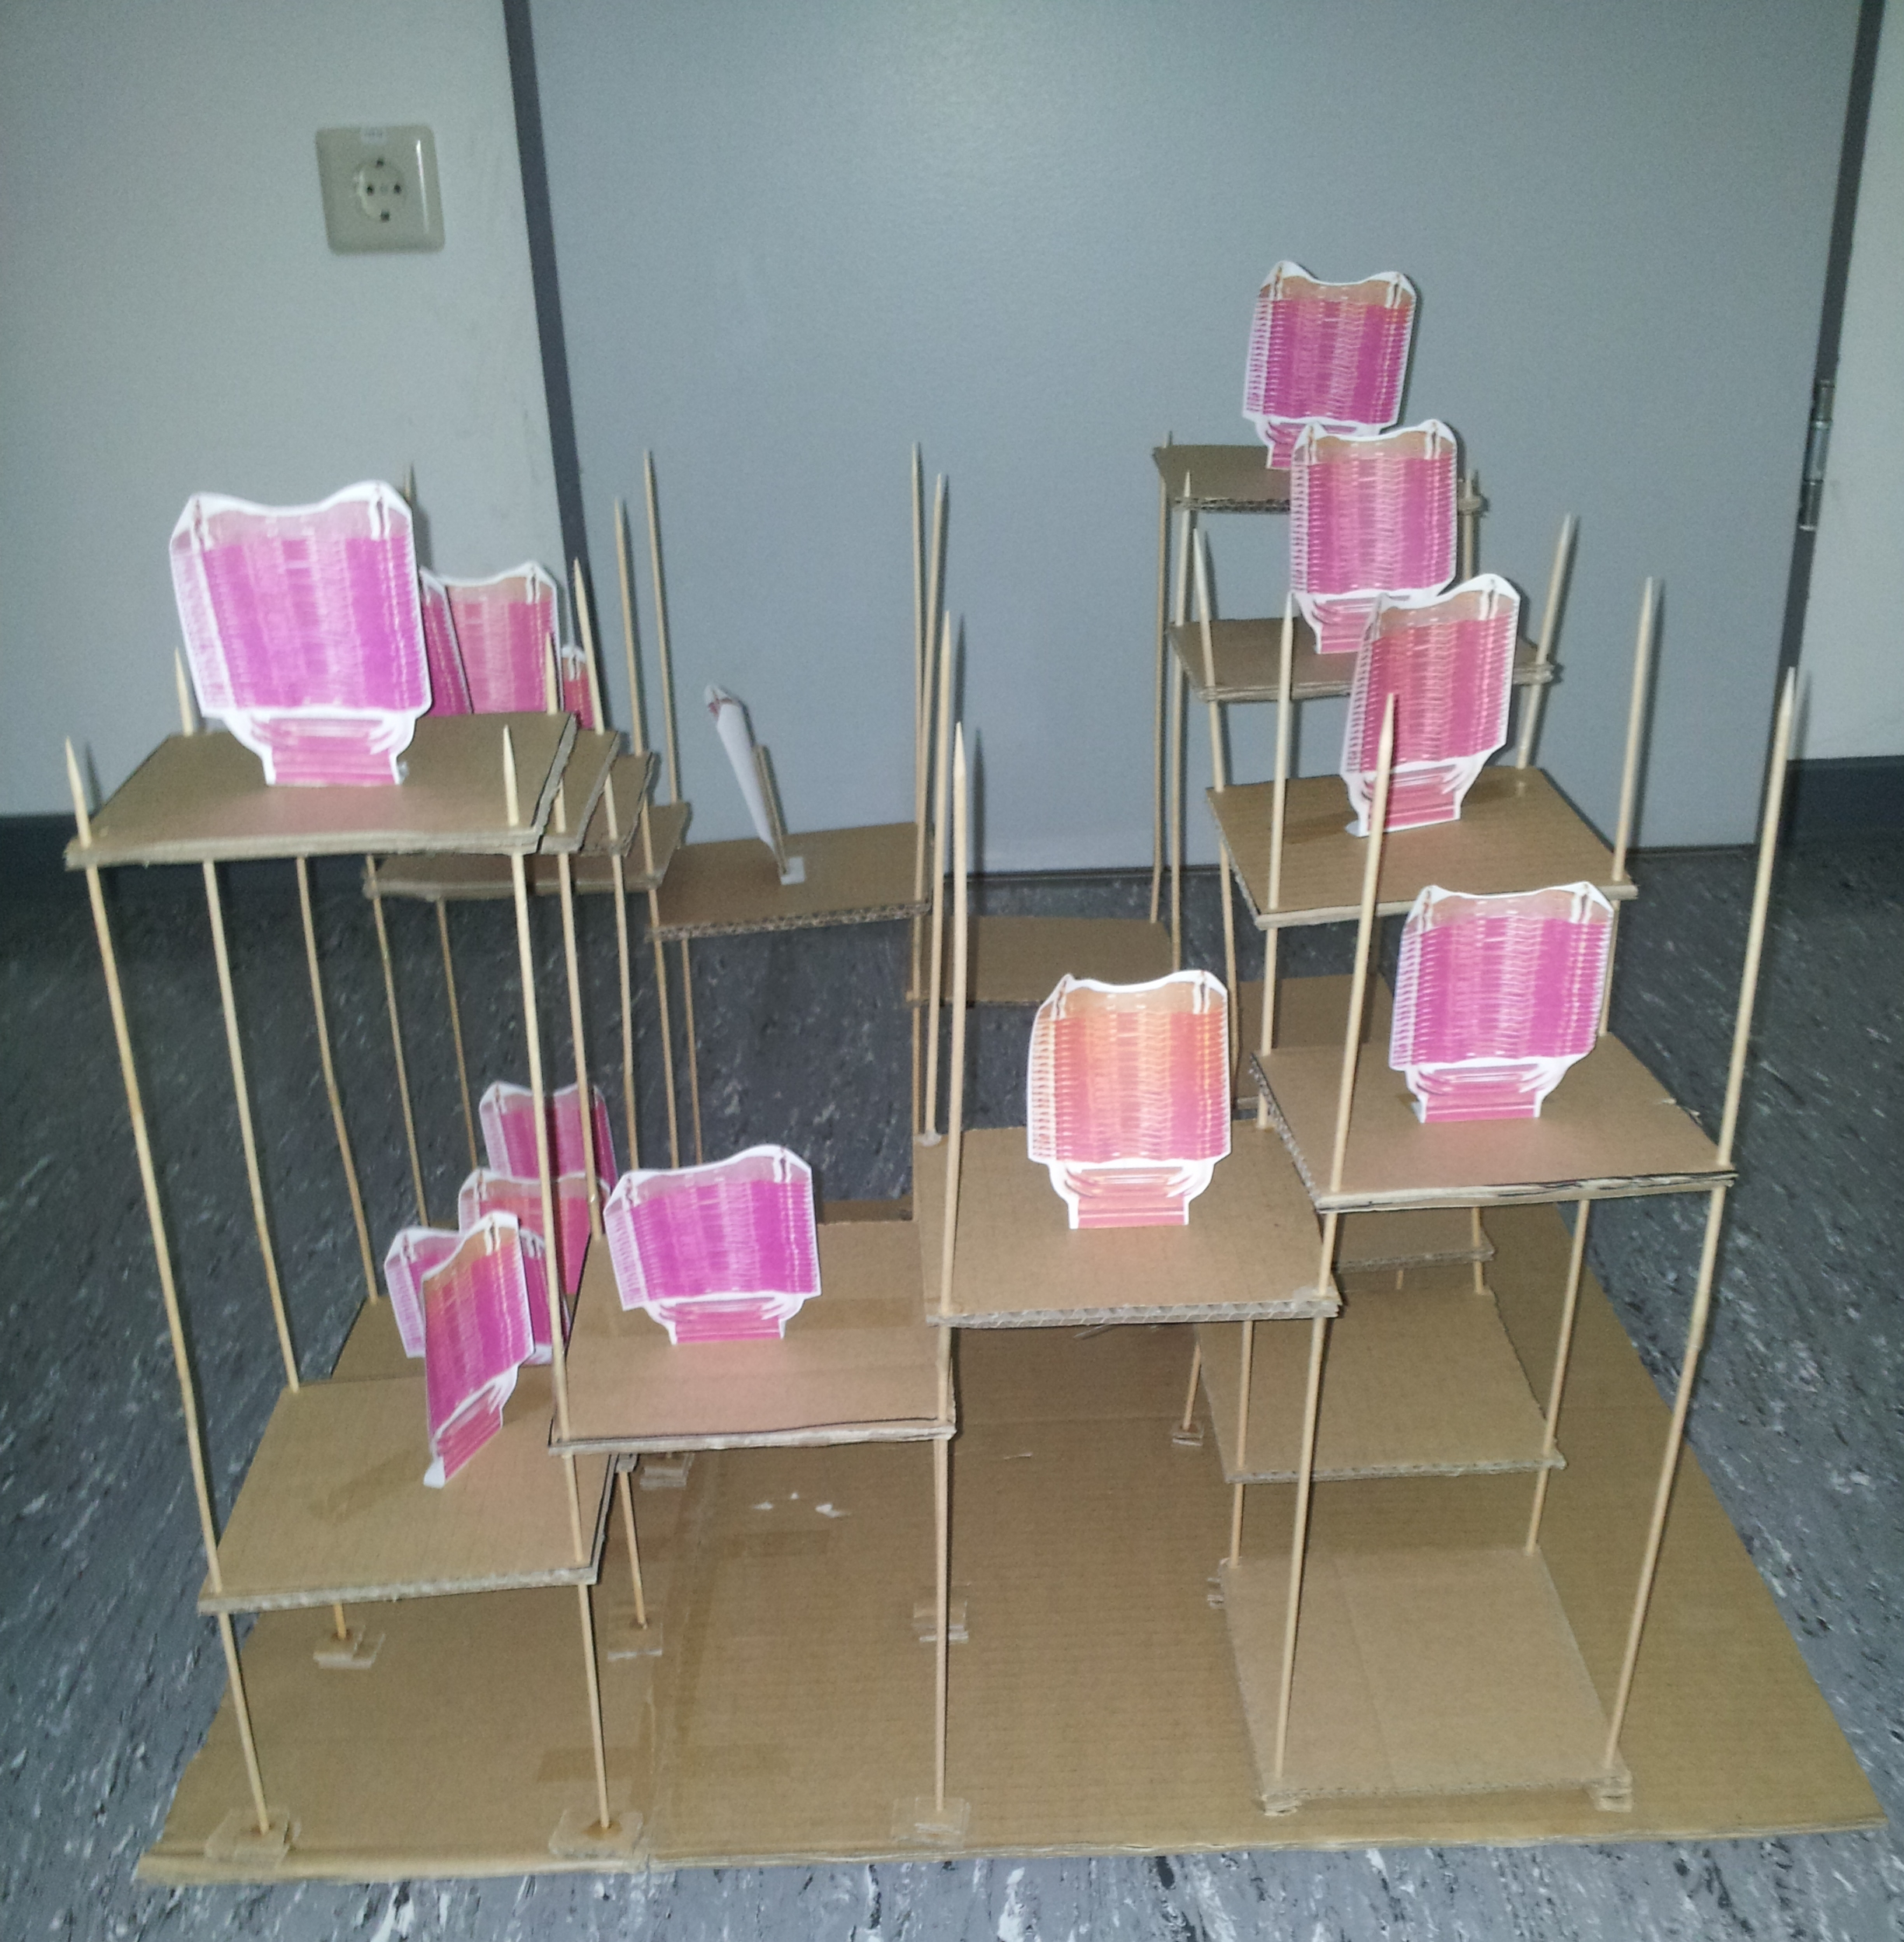
\includegraphics[scale=0.07]{./Bilder/20150929_133702-2.jpg}
\caption{Aufbau als Doppelhelix (Modell)}
    \label{fig:HWP_DoppelHelixModell}
\end{figure} 
\end{minipage}
\hfill
\begin{minipage}{0.45\textwidth}
 \begin{figure}[H]
  \centering
    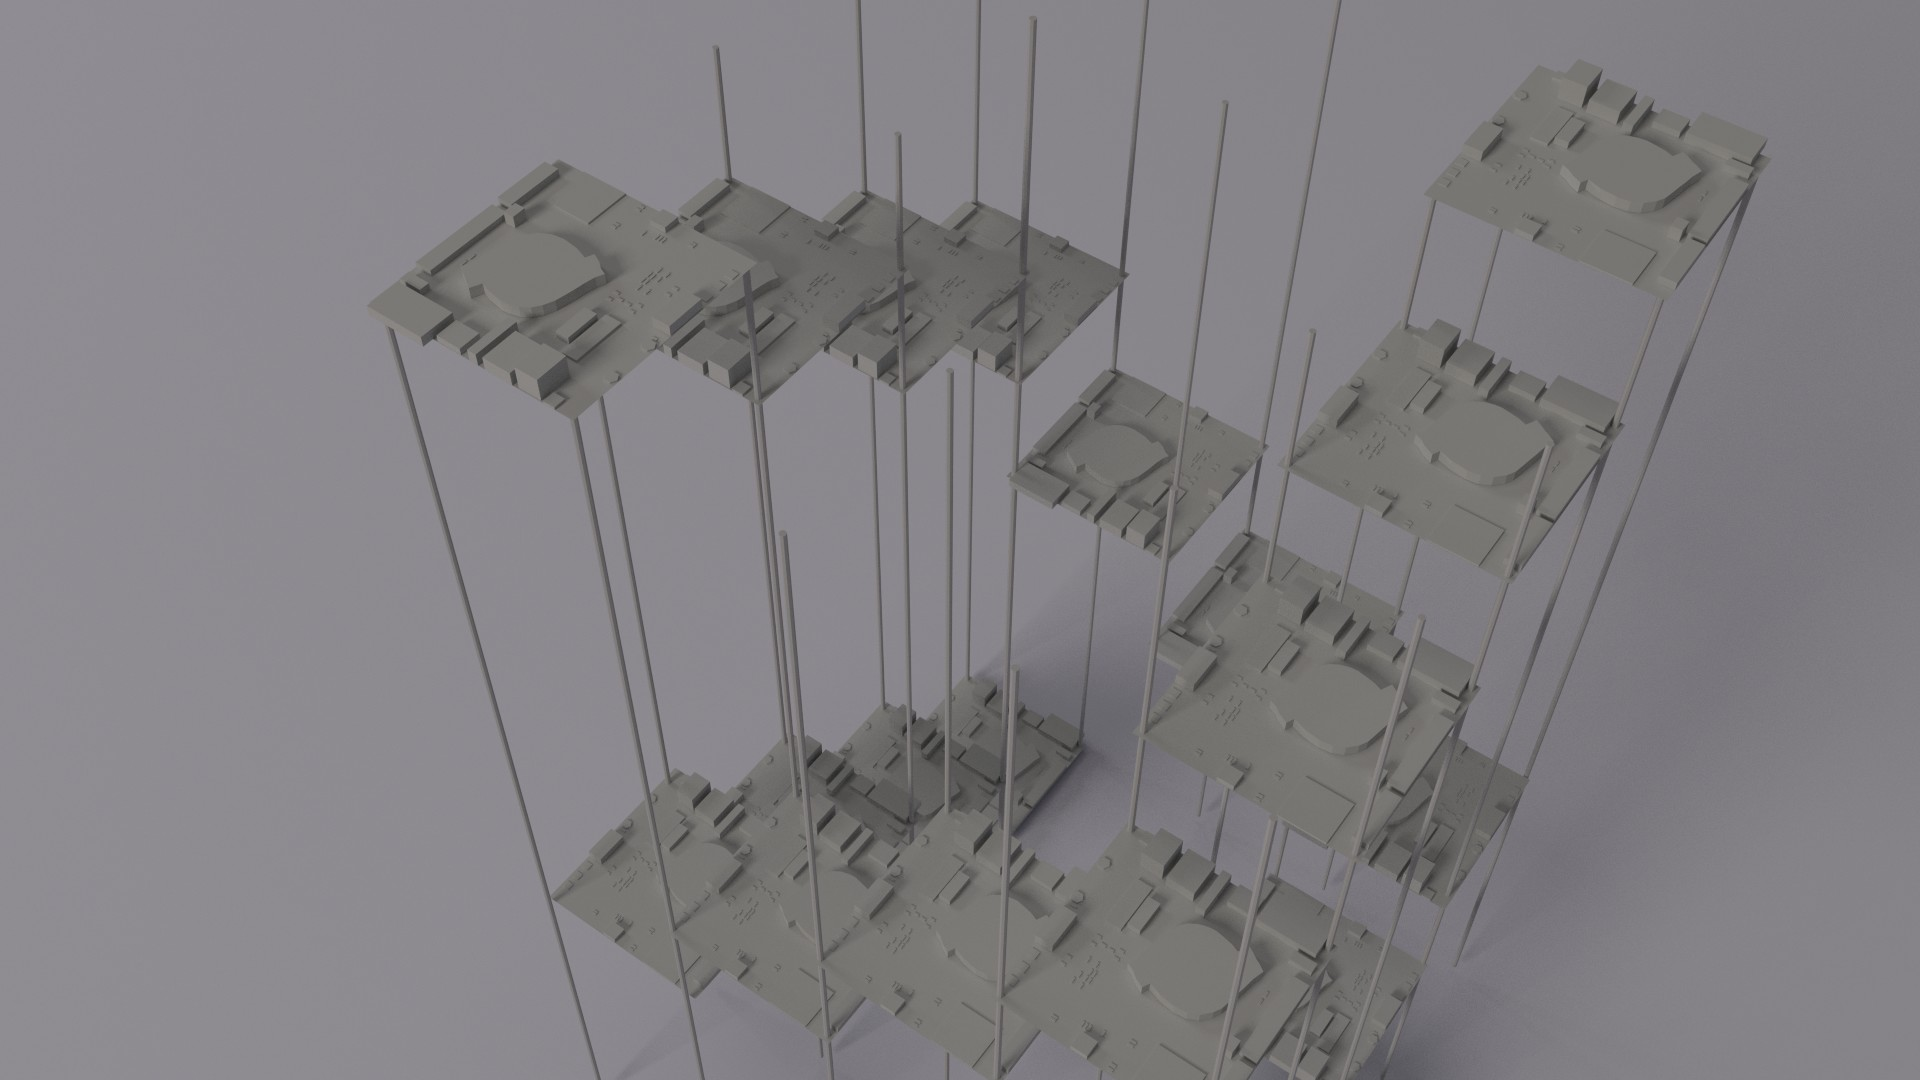
\includegraphics[width=\textwidth]{./Bilder/render3.jpg}
\caption{Computermodell für den Aufbau als Doppelhelix}
    \label{fig:HWP_DoppelHelixModellBlender}
\end{figure}
\end{minipage}


Um die Bildung von Wärmenestern zu vermeiden, hat man sich für die
Anordnung der Boards in einer Doppelhelix entschieden. Siehe Abbildung \ref{fig:HWP_DoppelHelixModell} und \ref{fig:HWP_DoppelHelixModellBlender}.
Besonders hinsichtlich Platzbedarf, und der vermeidung von Wärmenestern 
bietet dieser Aufbau große vorteile gegenüber der Stategie, die 
Rechenknoten in Schichten anzuordnen.
~\\~\\
Zusätzlich zur Anordnung der Knoten selbst ist die Auswahl der
sonstigen Hardware entscheident für die Stabile funktion des
Rechenclusters.\\
Um die Operation des Clusters besser überwachen zu können, hat man sich
für die Power-Distribution-Unit (PDU) [MODELLNAME] von APC entschieden, da
diese laut Hersteller eine genaue Messung des aktuellen Stromverbrauchs und
der Humidität unterstützt. Als Switch kommt der ``Small Business SG300-28''
von Cisco zum einsatz, da dieser durch geringen Stromverbrauch und
und viele Ports für die verwendung in einem grünen Supercomputer 
besonders geeignet ist.

\subsubsection{Planung der Stromversorgung}
Eine besondere Herausforderung stellt auch die 
Anordnung der Netzteile, der einzelnen Rechenknoten dar.
Um zu gewährleisten, dass sich durch das Aufheizen der Netzteile keine
Wärmenester bilden, wird eine spezielle Halterung verwendet.
Unter Nutzung moderner 3D-Druck Technologien, wie sie häufig in der 'Maker-Szene' eingesetzt werden,
wurde eine Halterung (\ref{fig:HWPabb5})entworfen und produziert, welche trotz geringem Materialaufwand eine sehr hohe Stabiliät 
und eine gute Luftzufuhr ermöglicht.~\\~\\
\begin{minipage}{\textwidth}
\begin{center}
	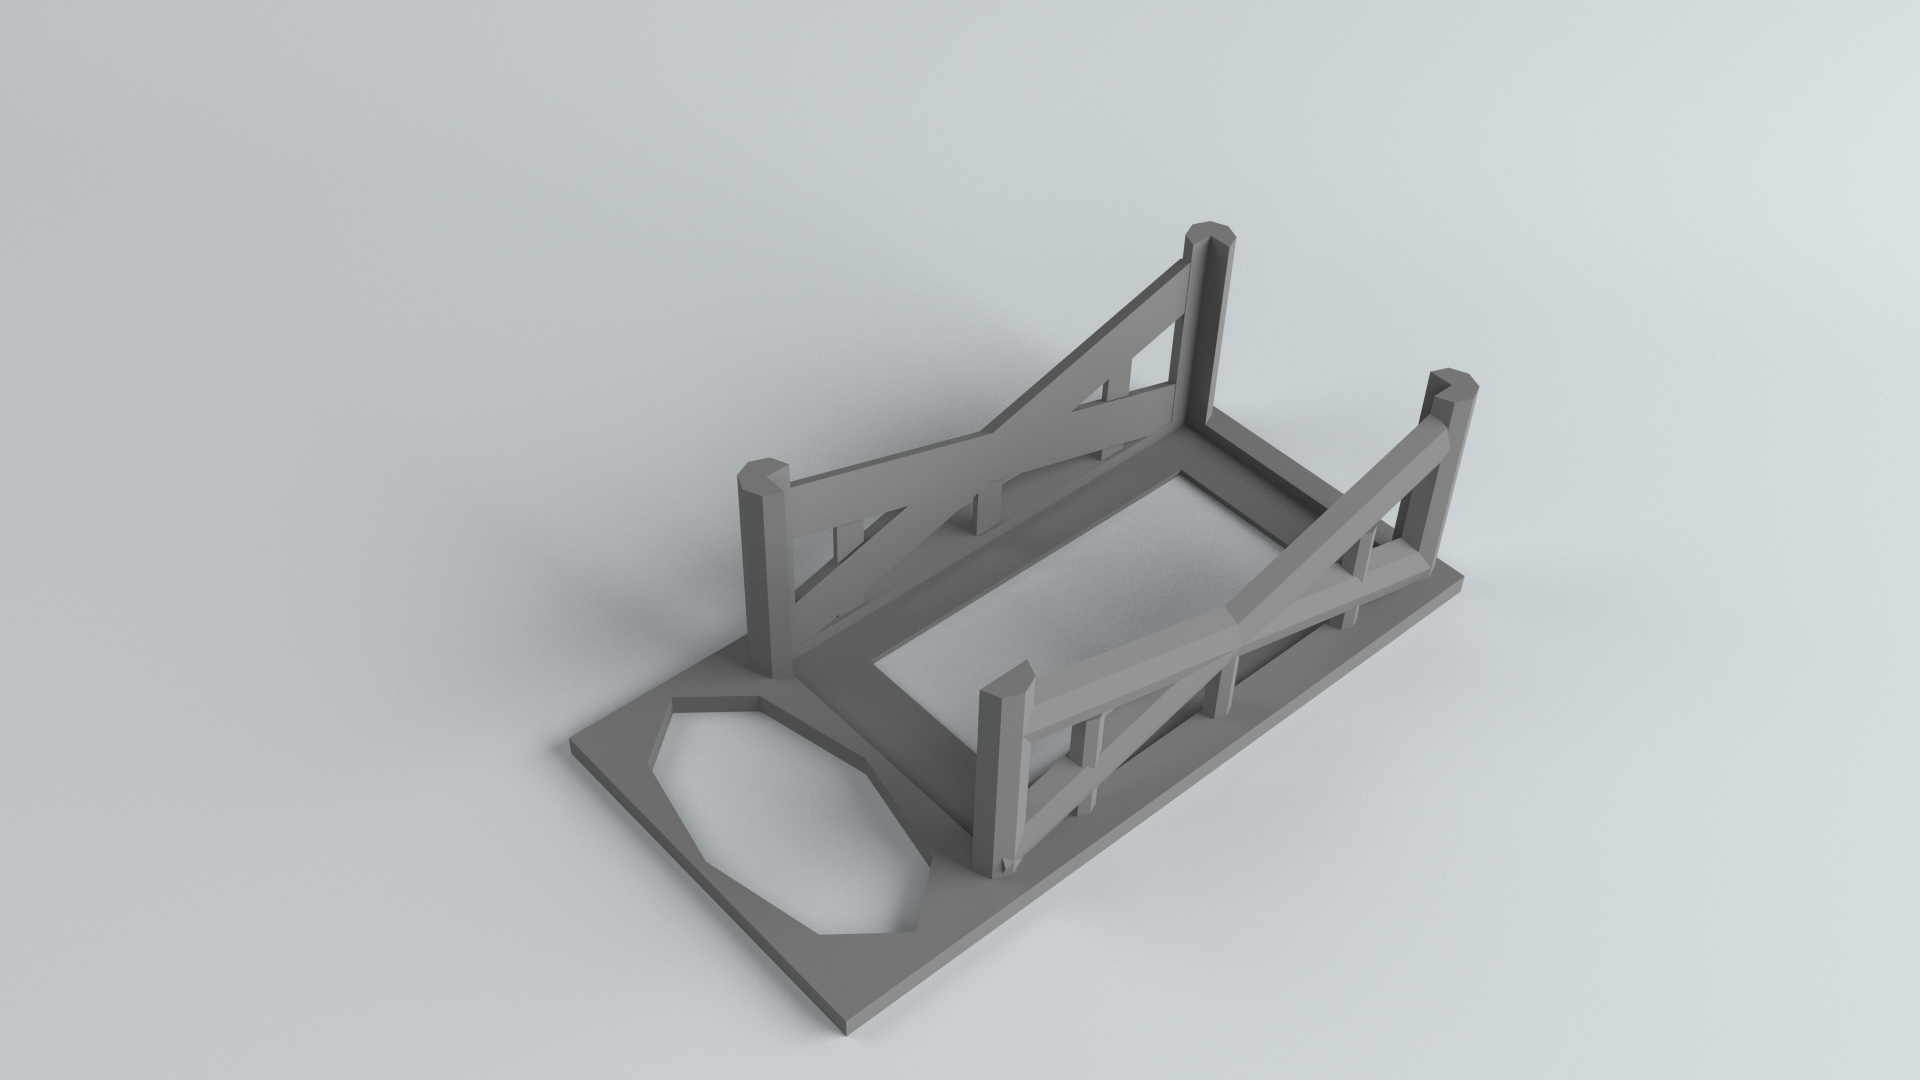
\includegraphics[width=0.5\textwidth]{./Bilder/Server-Aufbau/RenderPowerSupplyBox30.png}
	\captionof{figure}{Halterung für die Netzteile}
	%\captionof{figure}{Halterung für die Netzteile}
	\label{fig:HWPabb5}

\end{center}	
\end{minipage}
~\\

Hinsichtlich des Aspektes 'Green-Computing' ist es wichtig, ein Druckfilament zu verwenden, 
welches biokompatibel ist. Hierfür bietet sich der aus Maisstärke gewonnene Biokunststoff Polylactide (PLA) an.
Dieser hat einen Schmelzpunkt von $150^\circ\text{C}~\text{bis}~160^\circ \text{C}$
und ist daher ohne weiteres für die Halterung von Netzteilen verwendbar.



\subsection{Umsetzung}
Die Umsetzung des Aufbaus erfolgte aufgrund von guter Planung,
und modellgetreuer Umsetzung ohne Probleme.
Das fertig aufgebaute Cluster, sowie der verwendete Schlatplan 
sind in den Abbildungen \ref{fig:HWP_ICARUS_Server}
und \ref{fig:HWP_ICARUS_Schaltplan} dargestellt.~\\
\begin{minipage}{0.45\textwidth}
\begin{figure}[H]
  \centering
    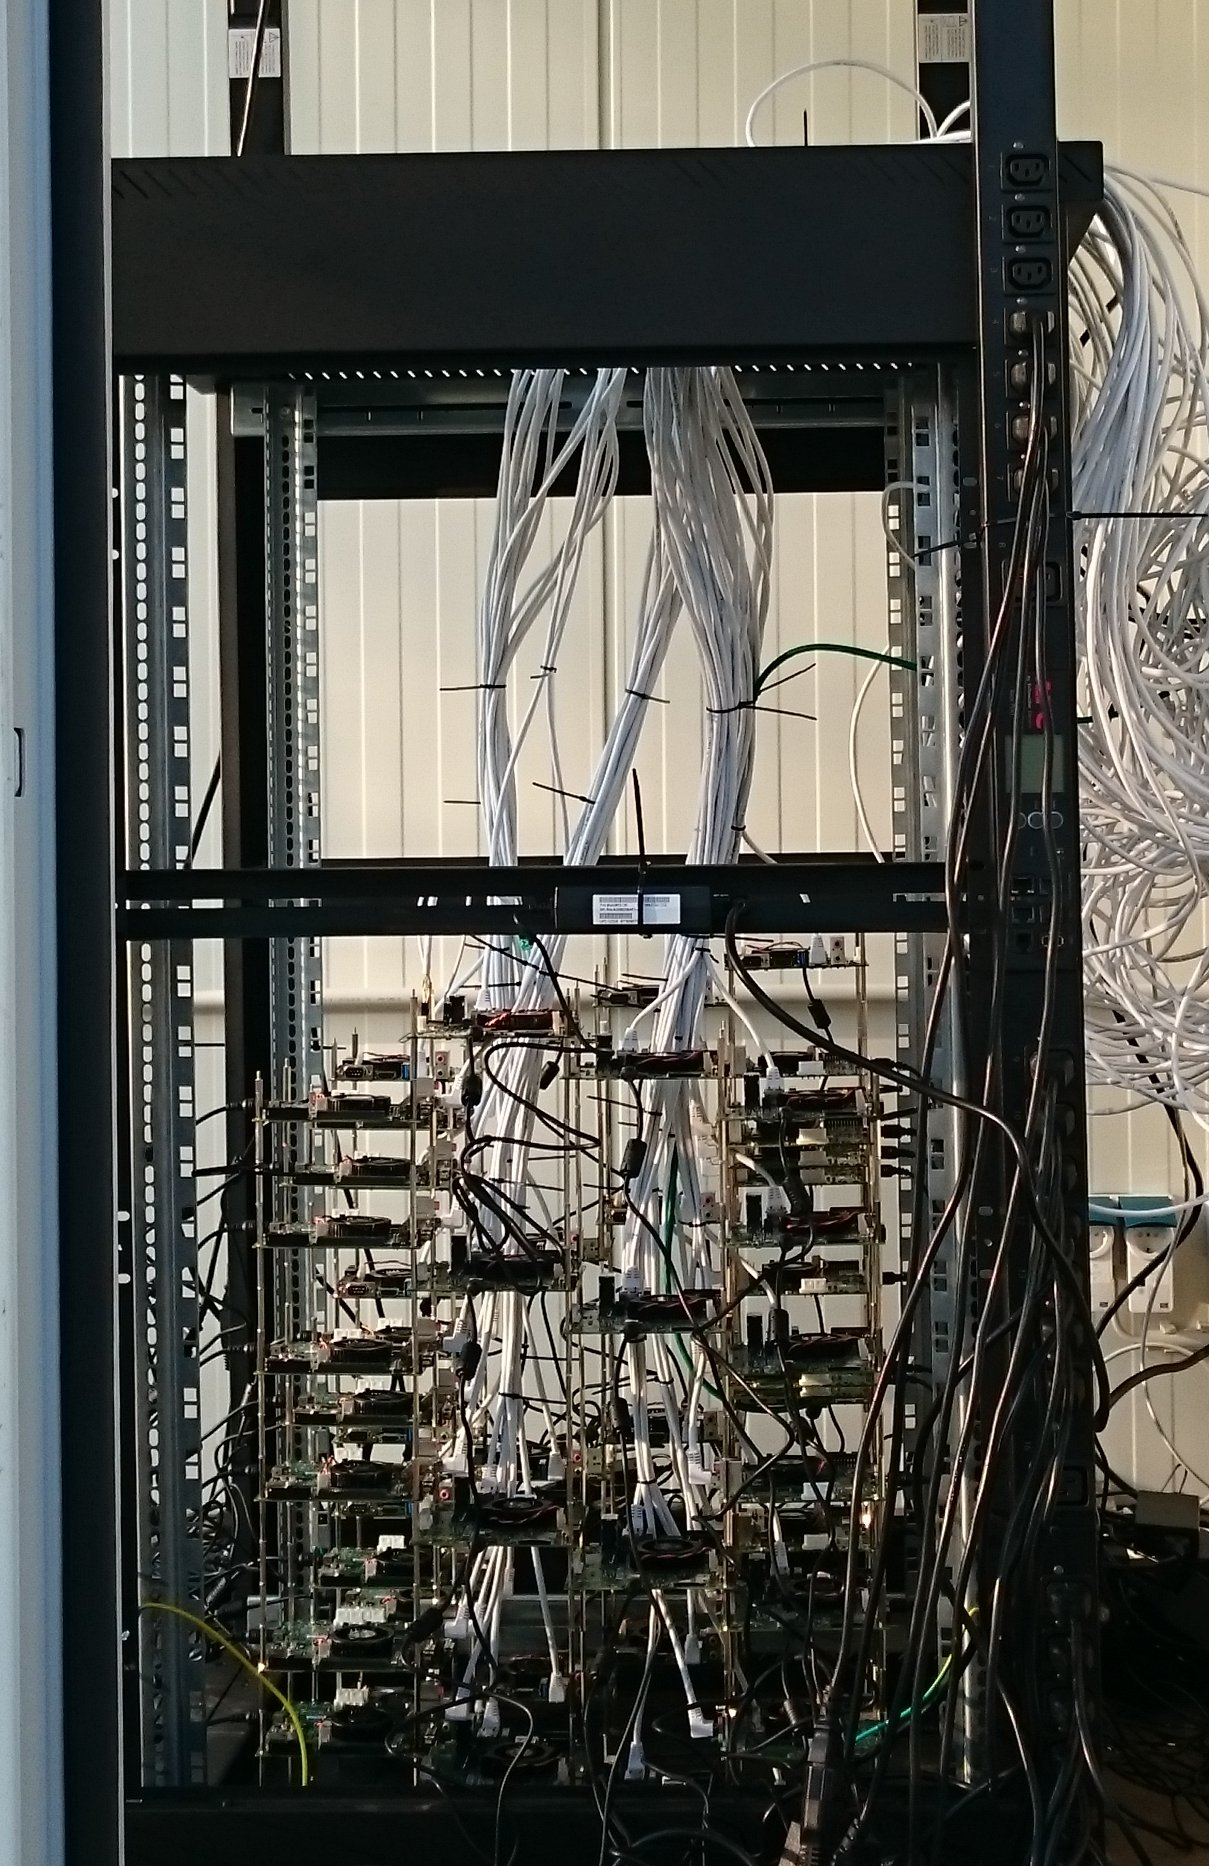
\includegraphics[width=0.5\textwidth]{./Bilder/Server-Aufbau/DSC_0020-small.JPG}
\caption{Aufbau des Servers}
    \label{fig:HWP_ICARUS_Server}
\end{figure} 
\end{minipage}
\hfill
\begin{minipage}{0.45\textwidth}
 \begin{figure}[H]
  \centering
    
\includegraphics[width=\textwidth]{./Bilder/EMPTY.jpg}
\caption{Schaltplan}
    \label{fig:HWP_ICARUS_Schaltplan}
\end{figure}
\end{minipage}




%\subsection{Wartung und Instandhaltung}
%\subsection{Dashboard} %(Ist gem dict.cc auch OK)
\subsection{Übersichtsseite}
Um das Monitoring und die Fernwartung des Clusters möglichst komfortabel zu bewerkstelligen, wurde ein Dashboard eingerichtet(\ref{fig:dashboardpic}). Hierfür ist die Hardware eines Raspberry Pi, der ersten Generation, ausreichend.
\subsubsection{Einrichtung Webserver}
Um die gemessenen Daten verwalten und darstellen zu können, wird auf dem Raspberry Pi ein LAMP-Server eingerichtet (Linux-Apache-MySQL-PHP). Die Daten werden folglich in der MySQL Datenbank abgespeichert und über PHP-Skripte ausgelesen und verarbeitet. Die Darstellung der Daten erfolgt mittels HTML, CSS und Javascript. Des Weiteren muss der Raspberry Pi so konfiguriert werden, dass erstens das Webinterface von außen einsehbar ist, und vor allem, dass auch von außen in die Datenbank geschrieben werden kann.

\begin{minipage}{\textwidth}

\begin{center}
	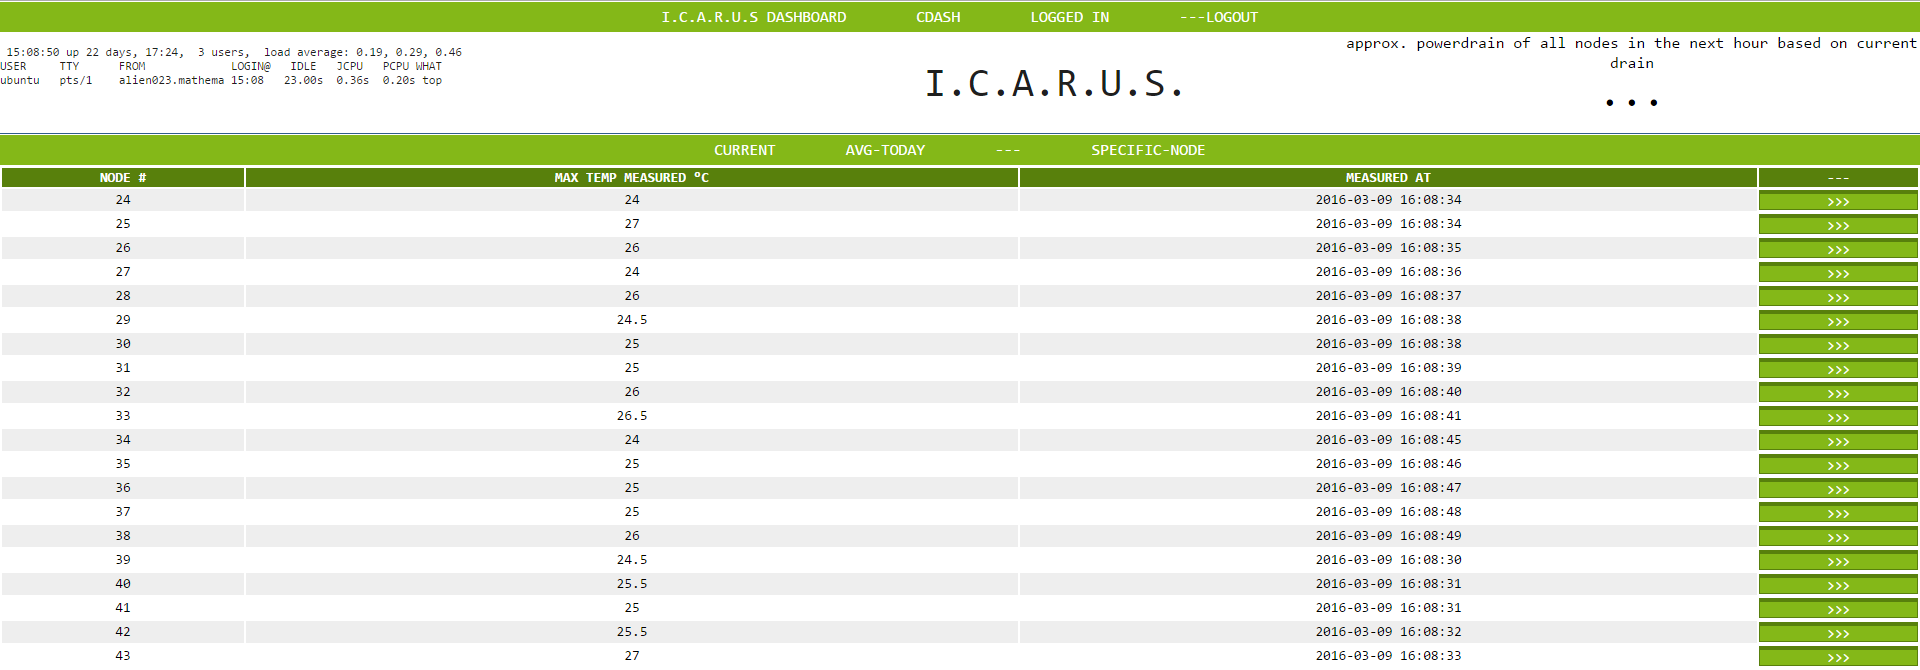
\includegraphics[width=0.7\textwidth]{./Bilder/Dashboard/Dashboard_frontend.png}
		\captionof{figure}{Dashboard Frontend}
	\label{fig:dashboardpic}

\end{center}	
\end{minipage}

\subsubsection{Sammeln der Messdaten}
Die Temperaturen können lokal auf den einzelnen Boards ausgelesen werden. Dies wird verwendet, um mittels C++ ein Programm laufen zu lassen, welches sich auf den einzelnen Rechenknoten nacheinander einloggt, die Temperatur Daten an verschiedenen Stellen des Jetson-Boards ausliest und anschließend zusammen in die MySQL-Datenbank auf dem Webserver einfügt.\\
Um die restringierte Hardware des Raspberry Pi's nicht zu überlasten, wird das Programm auf dem Gateway-Knoten des Clusters ausgeführt, weshalb der oben genannte Zugriff von außen des Raspberry Pi's wichtig ist. \\
Um qualitative Aussagen über die Energieeffizienz machen zu können wurde eine PDU angeschafft, mit welcher der Stromverbrauch der einzelnen Knoten messbar gemacht werden sollte. \\
--- kleiner Text bzgl alternativer Messmethoden folgt nach Donnerstag nach Gespräch mit Markus---\\

\subsubsection{Weitere Funktionen des Dashboards}
Die Aufgabe der Übersichtsseite beschränkt sich nicht nur auf das Sammeln und Anzeigen der Daten. Es soll auch die Fernwartung der einzelnen Knoten bezüglich der Stromzufuhr geregelt werden. Dies soll mittels SSH-Zugriff auf die PDUs bewerkstelligt werden, ist jedoch zur Veröffentlichung dieses Berichts noch in Entwicklung.
Des Weiteren wird ebenfalls mittels SSH-Zugriff und elementaren Linux-Befehlen die aktuell am Cluster angemeldeten Nutzer, sowie deren aktuell ausgeführten Programme, angezeigt.
